%%%%%%%%%%%%%%%%%%%%%%%%%%%%%%%%%%%%%%%%%%%%%%%%%%%%%%%%%%%%%%%%%%%%%%%%%%%%%%%%%%%%%%%%%%%%%%%%%%%%%%
%
%   Filename    : appendix_B.tex 
%
%   Description : This file will contain one of your appendices.
%                 
%%%%%%%%%%%%%%%%%%%%%%%%%%%%%%%%%%%%%%%%%%%%%%%%%%%%%%%%%%%%%%%%%%%%%%%%%%%%%%%%%%%%%%%%%%%%%%%%%%%%%%
\Section{Architectural Design}
\label{sec:appendixb}

\begin{figure}[h]                %-- use [t] to place figure at top, [b] to place at the bottom
   \centering                    %-- use this to center the figure
   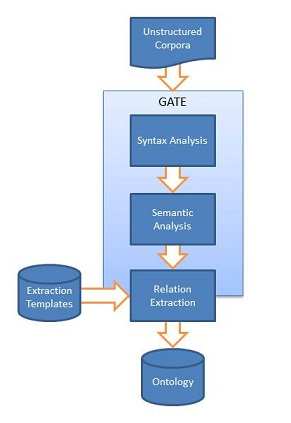
\includegraphics{archidesign.jpg}      %-- include image file named as "sinag1.eps" 
   \caption{Architectural Design}
    \label{fig:archidesign}
\end{figure}

Shown in \ref{fig:archidesign} is the architectural design for the relation extraction system to be developed. The process requires an unstructured corpora as an input, which in this case would be a children's story. It has been manually validated and modified to fit the tool requirements. Some modifications include the removal of dialogues. Once the input has already been form-fitted, it goes through GATE for syntax analysis. It first splits the corpora into tokens and sentences. The corpora is then passed to the tagger which annotates each word or symbol with their part-of-speech tags. GATE is then used to recognize the named-entities in the corpora. The named-entities are used later in relation extraction to determine whether a pair of entities fit the extraction templates. After syntax analysis, the corpora then goes into semantic analysis wherein the words' morphology and tense are annotated. The sentences are also chunked into phrases/clauses to accommodate concepts involving multiple words. Once all preprocessing to the corpora has been done, it goes through relation extraction wherein relations found in a sentence and across sentences are extracted. This uses the extraction templates. The extraction is done in two phases. The first phase is done through the JAPE Transducer where simple relations are tagged and extracted. The second phase involves the extraction of event-related relations. After extraction, simple inferencing will be done to ensure that final relations will not have proper nouns and become as general as possible. Lastly, the extracted relations are stored in an ontology similar to that of Picture Books. 



